\chapter{Theoretical Background}

\label{Chapter-Theoretical-Background}

The theoretical background of Machine Learning and Convolutional Neural Networks is being described below.

\section{Machine Learning}
Machine Learning, the name of which was first proposed in 1959 by Arthur Samuel \cite{Some-Studies-in-Machine-Learning-Using-the-Game-of-Checkers}, is a subset of Artificial Intelligence, a Computer Science (CS) field that studies algorithms and statistical models capable of performing specific tasks, such as prediction or decision making, without being explicitly programmed. Instead, sample data are used, also known as "training data", for the machine to "learn" to distinguish useful patterns on the input data capable of creating the needed output, e.g., decision or prediction. There are numerous approaches \cite{Machine-learning-Wikipedia} on the learning algorithms types, as well as on the model types used to get trained.

Such algorithm types, at the time of writing, include, but are not limited to:
\begin{itemize}
	\item \textbf{Supervised Learning:} Algorithms that learn by using "labeled" sample data, " containing both the inputs and their desired outputs for classification and regression.
	\item \textbf{Unsupervised Learning:} In contrast with the Supervised Learning, unlabeled sample data are used to discover structures that could group or cluster them.
	\item \textbf{Reinforcement Learning:} Algorithms responsible for taking actions in an environment, often also described as software agents, to maximize a specific metric, many of which use dynamic programming techniques.
	\item \textbf{Feature Learning:} Algorithms that by combining or even discarding features from the input samples, try to create a new, more useful set of features. One of the most popular algorithms of this category is Principal Components Analysis (PCA).
	\item \textbf{Anomaly Detection:} Algorithms that try to identify outlier samples, which are characterized by their significant difference compared to the majority of the data used. Such algorithms are often used in noise reduction, data mining, and even security and defense systems.
	\item \textbf{Association Rule Learning:} Algorithms that aim to discover strong relationships between features.
\end{itemize}

Such model types, at the time of writing, include, but are not limited to:
\begin{itemize}
	\item \textbf{Artificial Neural Networks (ANN):} Also known as Connectionist Systems, imitate the biological brain's neural networks.
	\item \textbf{Decision Trees:} Make assumptions about the input items' target value (the decision tree's leaves) via its observations (the decision tree's branches). When the target takes continuous values, the Decision Tree is called a Regression Tree.
	\item \textbf{Support Vector Machines (SVM):} Used for classification and regression, most\-ly famous as non-probabilistic, binary, linear classifiers. They can also be used for non-linear classification using the kernel trick.
	\item \textbf{Bayesian Networks:} Represented as directed acyclic graphs, they can include probabilistic relationships.
\end{itemize}

Nowadays, most industries have already used Machine Learning in some sort, indicating the significance and variety of its capabilities. It is estimated \cite{Machine-Learning-Applications} that by the year 2021, AI and ML spending will reach 57.6 Billion USD. Its applications include but are not limited to \cite{Top-Machine-Learning-Applications-in-2019} \cite{Roundup-Of-Machine-Learning-Forecasts-And-Market-Estimates}, web page ranking, image recognition, email filtering, and spam detection, database mining, handwriting recognition, speech recognition, natural language processing, computer vision, image/video/text/speech generation, personalized marketing, traveling, dynamic pricing, healthcare, facial and fingerprint recognition and intrusion detection.

\section{Artificial Neural Network}
It is widely accepted that the brain's most exceptional ability is pattern recognition, which is used to combine "data" from the organism's senses in a way to better understand its environment. Artificial Neural Networks (ANN), a highly popular sub-field of Machine Learning, try to imitate the brain's structure to solve such problems, a structure that has been developing and proving its capabilities for thousands of years.

While ANNs are inspired by biological neural networks, they are not identical. A neural network is a collection of connected neurons, through which electrical signals from sensor organs or other neurons are passed and processed. A biological neuron is comprised of four main parts; Dendrites, Cell body, Axon, and Synaptic terminals (Figure \ref{fig:Standard-structure-of-a-biological-neuron}). A Dendrite and its Dendritic branches are used as the neuron's input, where sensors or other neurons get connected. A neuron can have multiple Dendrites. The neuron's cell body collects all the input signals and applies an "activation" function to create the output signal. Afterward, the output signal is transported through the Axon and distributed to the next neurons through the Synaptic terminals. The Synaptic terminals to Dendrites connections are called Synapses.

\begin{figure} [H]
	\centering
	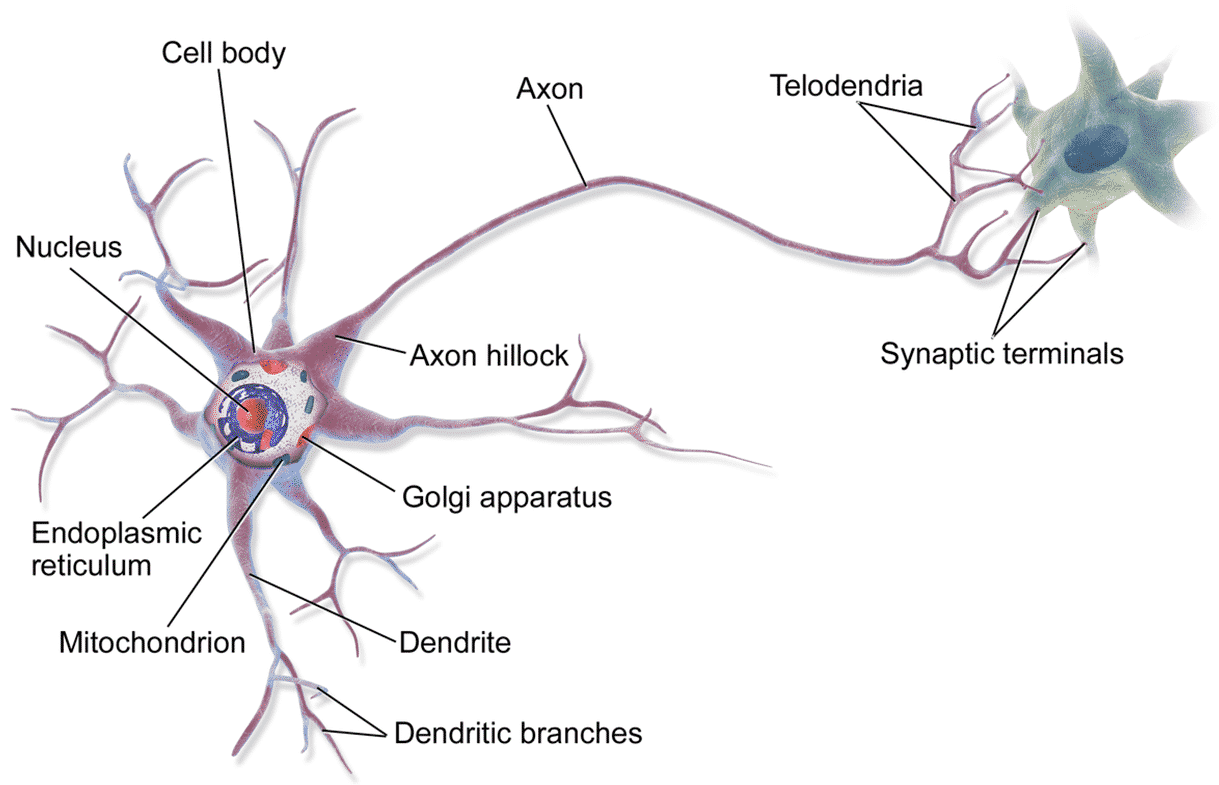
\includegraphics[scale=0.25]{Images/Biological-Neuron.png}
	\decoRule
	\caption[Standard structure of a biological neuron]{Standard structure of a biological neuron: \href{https://nurseslabs.com/nervous-system/}{URL}}
	\label{fig:Standard-structure-of-a-biological-neuron}
\end{figure}

\subsection{ANNs Basic components} \label{subsection:ANNs-Basic-components}
Similarly to the biological neural networks, an ANN can be represented as a directed, weighted graph (Figure \ref{fig:simplified-neural-network-graph}), whose vertices represent the biological neurons' cell bodies and its edges the biological synapses. The electrical signal used in biological neurons can be represented as a real number, and their outputs can be calculated by some non-linear function of the inputs' weighted sum. Each edge typically can have a weight, set during the training process, which amplifies or weakens the vertex's signal.

\begin{figure} [H]
	\centering
	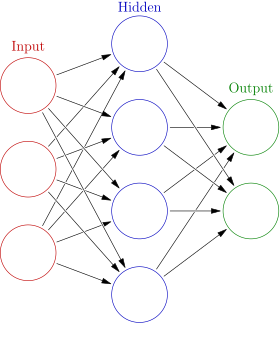
\includegraphics[scale=0.5]{Images/simplified-neural-network-graph.png}
	\decoRule
	\caption[Activation Function Graphs]{Simplified Neural Network Graph: \href{https://en.wikipedia.org/wiki/Artificial_neural_network}{URL}}
	\label{fig:simplified-neural-network-graph}
\end{figure}

\subsubsection{Neuron}
A neuron receives real numbers as inputs, which are combined with their internal state, also known as activation, using an activation function and an optional threshold to produce the neuron's output.

\subsubsection{Connections and Weights}
Each neuron can be connected with multiple other neurons to be used as inputs and to feed them with its output. Each connection is characterized by its weight, which represents its relative importance.

\subsubsection{Propagation Function}
The propagation function calculates the weighted sum of each neuron's inputs and adds a bias term.

\subsubsection{Activation Function}
The activation function receives the propagation function's result and applies a transformation, which creates the neuron's final output. There are a lot of different activation functions, with specific characteristics for the training and inference process. However, they all provide a smooth and differentiable transition as the input values change. The most commonly used ones are shown below \cite{Activation-Function-Wikipedia}.
\begin{itemize}
	\item \textbf{Identity:} $f(x) = x$\\
	No transformation is applied.

	\item \textbf{Binary Step:} $
		      f(x) =
		      \begin{cases}
			      0 & x \leq 0 \\
			      1 & x > 0
		      \end{cases}
		  $\\
		  While being the original activation function developed when neural networks were invented, it is no longer used as it is incompatible with backpropagation. Backpropagation is the process of updating the weights during the training phase using the gradient descent algorithm. The binary step function is not convex; hence, gradient descent is unable to find a local minimum.

	\item \textbf{Logistic (Sigmoid or Soft step):} $
		      f(x) = \sigma(x) = \frac{1}{1 + e^{-x}}
		  $\\
		  Often used, however, in real-world neural networks, it is avoided due to the vanishing gradient problem \cite{The-Vanishing-Gradient-Problem-During-Learning-Recurrent-Neural-Nets-and-Problem-Solutions}.

	\item \textbf{TanH:} $
		      f(x) = tanh(x) = \frac{e^{x} - e^{-x}}{e^{x} - e^{-x}}
		  $\\
		  Same as Logistic.

	\item \textbf{Rectified Linear Unit (ReLU):} $
		      f(x) =
		      \begin{cases}
			      0 & x < 0 \\
			      x & x > 0
		      \end{cases}
		  $\\
		  The most popular activation function, due to its fast backpropagation speeds, its low penalty on generalization accuracy, and its resistance to saturation conditions \cite{ImageNet-Classification-Using-Binary-Convolutional-Neural-Networks}.

	\item \textbf{Softmax:} $
		      f_i(\textbf{x}) = \frac{
		      e^{x_i}
		      }{
		      \sum_{j=1}^{J}e^{x_j}
		      }
		  $, for i = 1, ..., J\\
		  Commonly used as a final output activation function for multiclass classification. It normalizes the output to [0, 1], and makes its sum equal to 1. After this transformation, the i-th output's value designates the probability of the input to be the class i.
\end{itemize}

\begin{figure} [H]
	\centering
	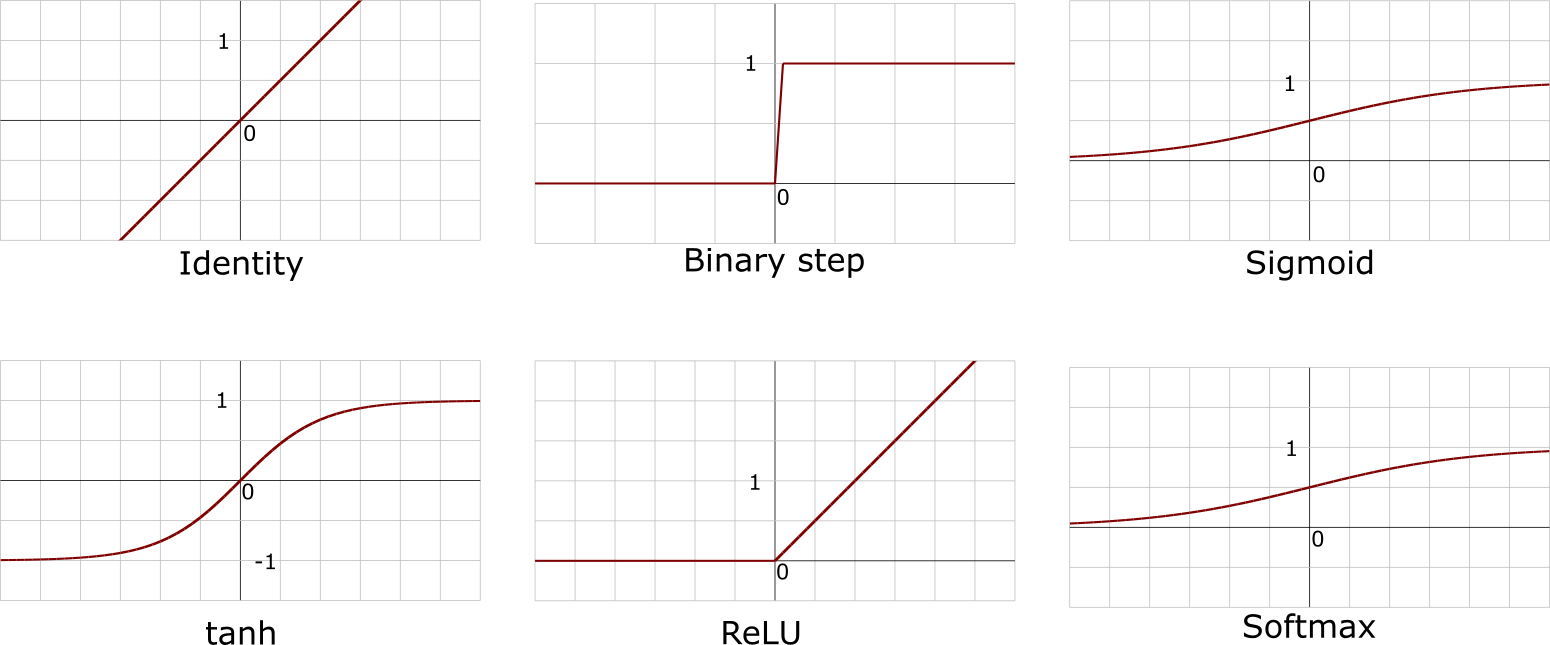
\includegraphics[width=\textwidth]{Images/Activation_functions.png}
	\decoRule
	\caption[Activation Function Graphs]{Activation Function Graphs}
	\label{fig:activation-functions}
\end{figure}

\subsection{Organization}
An ANN's neurons are typically organized into groups, called layers, in which each neuron has the same distance from the inputs as all the other neurons of its group. The input layer is the layer that gets as inputs the external data, and the output layer, the last layer in the graph, is the one that produces the final output results. Any in-between layer is called a hidden layer. An ANN is called a Deep Neural Network (DNN), when, by convention, it has three or more hidden layers.

\subsection{ANN Architectures}
There are many ANN architectures, each one serving different use cases. They are separated into two main groups, Feedforward networks and Recurrent networks \cite{Types-of-Artificial-Neural-Networks}.

\subsubsection{Feedforward Networks}
The basic idea with the feedforward networks is that the data flows from the input layer through the hidden layers to the output layer without any cycles, so they can be represented as directed, acyclic graphs. Some architectures of this group are:
\begin{itemize}
	\item Multiclass Perceptron
	\item Group method of data handling
	\item Autoencoder
	\item Probabilistic
	\item Time delay
	\item Convolutional
	\item Deep stacking network
\end{itemize}

\subsubsection{Recurrent Networks}
Recurrent Neural Networks (RNN), similarly to the Feedforward networks, data flows from the input layer through the hidden layers to the output layer. However, they allow for data cycles, in other words, outputs of the $layer_n$ can be fed to the inputs of the $layer_{n-1}$, so they can be represented as directed, cyclic graphs. Some architectures of this group are:
\begin{itemize}
	\item Fully recurrent
	\item Simple recurrent
	\item Reservoir computing
	\item Long short-term memory
	\item Bi-directional
	\item Hierarchical
	\item Stochastic
	\item Genetic Scale
\end{itemize}
For every ANN Architecture, there are specific types of layers that apply different kinds of mathematical operations on their input data. Each layer type has characteristics on the way its mathematical operations are applied to its input. Those characteristics are generally called hyperparameters. For example, in a Fully-Connected layer, a hyperparameter is its number of outputs. Hyperparameters are set by the engineers during the training phase, which are fine-tuned, concerning the application's input data.

This work is focused on the Convolutional Neural Networks (CNN), which are described in detail below.

\section{Convolutional Neural Networks}
Convolutional Neural Networks (CNNs) are deep feedforward neural networks that specialize in processing data with grid-like topologies and are typically used in visual imagery analysis. They are simple neural networks that, for at least one of their layers, use the convolution mathematical operation instead of the general matrix multiplication \cite{Goodfellow-et-al-2016}.

CNNs imitate the brain's visual cortex, which is the area responsible for the visual processes. Cortical neurons cover small areas of the visual field, with partial overlaps resulting in full visual field coverage.

CNNs most significant advantage over other image classification algorithms is their little need for pre-processing, meaning that their filters are learned during the training phase while using traditional algorithms, they have to be hand-engineered.

Some of their applications are image and video recognition, image classification, object detection, recommendation systems, medical image analysis, natural language processing, and financial time series \cite{Convolutional-neural-networks-wikipedia}.

\subsection{Structure}
A typical CNN consists of two parts. The first part includes multiple convolutional and pooling layers, which extract features from the given input. The second part, also known as the classifier, includes multiple fully connected layers, which classify the given input using the features extracted from the first part (Figure \ref{fig:typical-cnn-architecture}).

\begin{figure} [H]
	\centering
	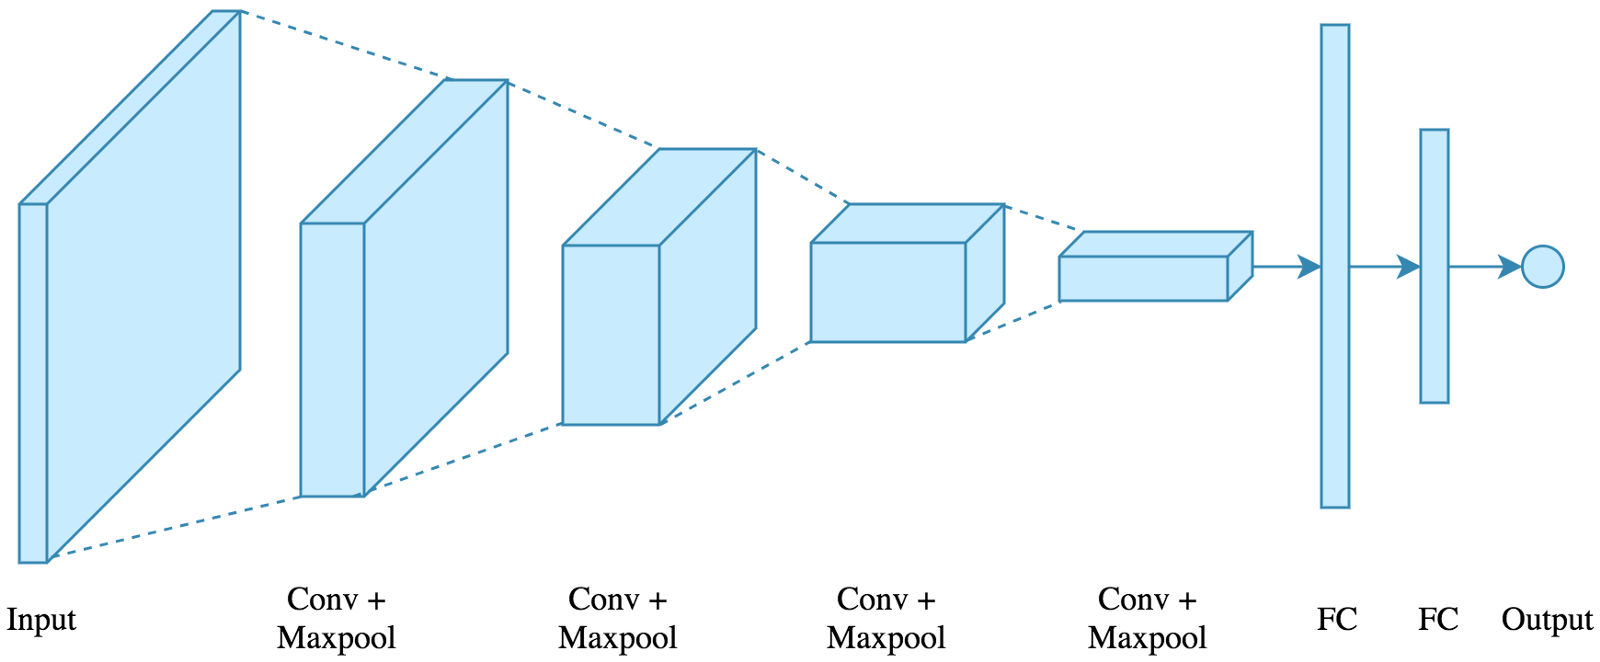
\includegraphics[width=\textwidth]{Images/typical-cnn-architecture.png}
	\decoRule
	\caption[Typical CNN Architecture]{Typical CNN Architecture - First five layers (Convolution + Max Pooling layers) used for feature extraction, last three layers (Fully-Connected) used for classification, also called the classifier: \href{https://www.kaggle.com/mauddib/digit-recogniser-tutorial-using-a-cnn-tensorflow}{URL}}
	\label{fig:typical-cnn-architecture}
\end{figure}

The input data is typically structured as multidimensional arrays, also known as tensors. For example, if the input data are RGB images, then the input tensor's shape is (number of images) x (image width) x (image height) x (image depth), where image depth is called the image's color channels, in this example 3 channels. Moreover, the input data can also be grayscale images or even hyperspectral images. Hyperspectral images have multiple color channels, even in the non-visible for the human eye spectrum, with applications including the medical and space fields. There are also implementations such as 1D and 3D CNNs, but this work examines 2D CNNs only.

The trainable parameters (weights and biases) needed for the computation are initially assigned random values \cite{Practical-recommendations-for-gradient-based-training-of-deep-architectures}, rendering the network useless. However, during the training phase, using the backpropagation process \cite{Learning-internal-representations-by-error-propagation}, those weights are being optimized to form features from the training set. The trainable parameters are also considered to be shared \cite{Generalization-and-network-design-strategies}, meaning that the same parameters are to be used in the entirety of the input data, dramatically decreasing their number and consequently their memory footprint and also increasing the network robustness against overfitting.

As stated above, there are three types of layers used in 2D CNNs; Convolutional, Pooling, and Fully-Connected layers. Each layer is being described below.

\subsubsection{Convolutional Layer}
A convolutional layer creates and outputs a similarity map between the input data and the convolution's filters, also known as kernels. More specifically, every filter is convolved across the input's width and height, producing their dot product. The result is multiple two-dimensional arrays, whose each cell holds the similarity of each filter to some spatial position in the input.

Each filter is a specific type of feature, depending on the training set. For example, in image classification, a filter can be a rough shape of cats' mustaches, so that after the convolution, it can be indicated if they are contained somewhere in the input image. If they are, then, to some probability defined during the training phase, there might be a cat in the input image.

Each convolutional layer is defined by its hyperparameters. Those are:
\begin{itemize}
	\item \textbf{Kernel size:} The width and height of the kernels' (filters') size, typically, small\-er than the given input.
	\item \textbf{Output channels:} The number of feature maps to be created as outputs. Consequently, the number of kernels used in this operation also equals the output channels number.
	\item \textbf{Stride:} The number of pixels to be skipped horizontally and vertically in each partial convolution. Typically, this number does not differ between the two dimensions.
	\item \textbf{Zero padding:} There might be a need for zero-padding the input to include as much data as possible in the final computation. There are three different ways of padding:
	      \begin{itemize}
		      \item \textbf{Valid:} No padding is applied; some data may not be included in the computation.
		      \item \textbf{Same:} Applies the amount of padding needed to result in the same width and height as the input.
		      \item \textbf{Full:} Applies padding on the input's edges with a specified number of pixels per dimension.
	      \end{itemize}
\end{itemize}

The mathematical expression of the convolution operation is defined bellow (Equation \ref{eqn:convolution}) and visualized on Figure \ref{fig:convolution-operation}.

Let \emph{I} be the input with \emph{C} channels, \emph{H} height and \emph{W} width, and let \emph{K} be the kernels with \emph{N} number of kernels, \emph{C} channels, \emph{KH} height and \emph{KW} width. Also, let \emph{B} be the bias with K values, and let \emph{S} be the stride size and \emph{P} be the padding size. So the convolution operation's output, \emph{Out}, is defined as:
\begin{equation}
	% Todo: fix overfull hbox
	I_{padded}(c, i, j) = \begin{cases}
		0,                  & i \in [1, P], j \in [1, P]                         \\
		I(c, i - P, j - P), & i \in [P + 1, P + 1 + H], j \in [P + 1, P + 1 + W] \\
		0,                  & i \in [H + 1, H + 1 + P], j \in [W + 1, W + 1 + P] \\
	\end{cases}
\end{equation}

\begin{equation}
	OH = \frac{H + 2P - KH}{S} + 1
\end{equation}

\begin{equation}
	OW = \frac{W + 2P - KW}{S} + 1
\end{equation}

\begin{equation}
	\label{eqn:convolution}
	% Todo: fix overfull hbox
	\begin{split}
		Out(k, i, j) = B(k) +
		\sum_{c = 1}^{C} \sum_{kh = 1}^{KH} \sum_{kw = 1}^{KW}
		I_{padded}(c, kh + i * KH, kw + j * KW) K(k, c, kh, kw),\\
		\mbox{for k = 1, 2, ..., C},\\
		\mbox{for i = 1, 2, ..., OH},\\
		\mbox{for j = 1, 2, ..., OW}\\
	\end{split}
\end{equation}

\begin{figure} [H]
	\centering
	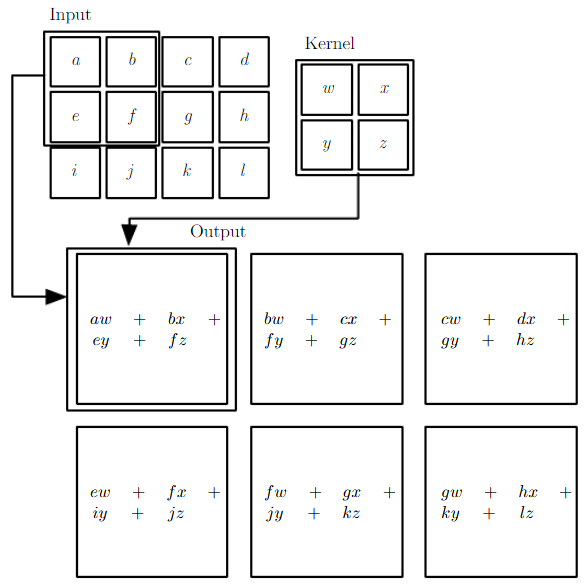
\includegraphics[scale=0.6]{Images/CNNArchitectures/convolution-operation.png}
	% 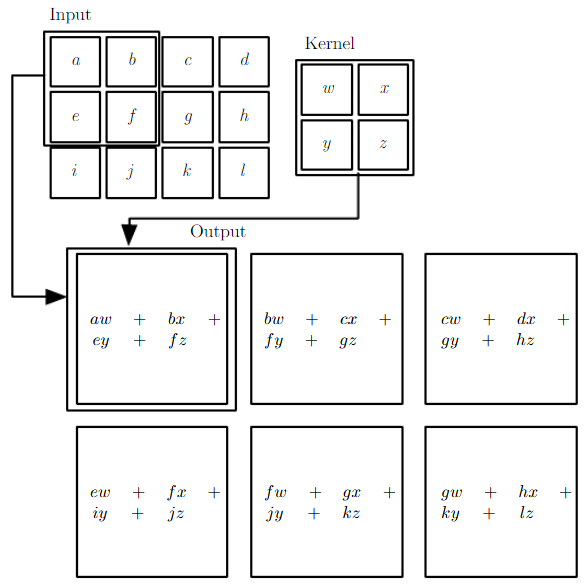
\includegraphics[width=\textwidth]{Images/CNNArchitectures/convolution-operation.png}
	\decoRule
	\caption[Convolution Operation]{Convolution Operation - A 2x2 Kernel filter is applied on the 4x3 example input matrix with stride 1 and valid padding. Figure from \cite{Goodfellow-et-al-2016}.}
	\label{fig:convolution-operation}
\end{figure}

Nowadays, most applications might require multiple Convolutional layers to extract useful features from their complex inputs. Deeper architectures, in general, create more detailed characteristics. Furthermore, activation functions can be interjected between adjacent Convolutional layers to enhance the network's nonlinearity. Activation functions can make the network function as a universal function approximator \cite{Approximation-capabilities-of-multilayer-feedforward-networks}.

\subsubsection{Pooling Layer}
A pooling layer sub-samples its input to decrease the computation footprint needed for the next layers and make the network more prone to over-fitting. It reduces the input dimensions by combining multiple neurons into a single neuron. Max-Pooling layers combine groups of neurons by outputting their maximum value. Average-Pooling layers combine groups of neurons by outputting their average value.

Similarly to the convolutional layer, a pooling layer slides a window of some size, called kernel size, across the input data. The data to be combined are those that the sliding window has selected. In 2D CNNs, the pooling layers have 2D windows; the channels are not combined.

A pooling layer can be local, combining small groups of neurons, which means that the layer's kernel size is small compared to the input size. It can also be global, combining the whole input to a single neuron.

Each pooling layer is defined by its hyperparameters. Those are:
\begin{itemize}
	\item \textbf{Kernel size:} The kernel's (sliding window's) width and height.
	\item \textbf{Stride:} The number of pixels to be skipped horizontally and vertically in each slide. Typically, this number does not differ between the two dimensions.
\end{itemize}

The mathematical expression of the average-pooling operation (Equation \ref{eqn:avg-pooling}) and max-pooling operation (Equation \ref{eqn:max-pooling}) is defined and visualized (Figure \ref{fig:max-pooling-operation}) bellow.

Let \emph{I} be the input with \emph{C} channels, \emph{H} height and \emph{W} width, let \emph{KH} be the kernel's height, let \emph{KW} be the kernel's width, and let \emph{S} be the stride size. So the pooling operations are defined as:
\begin{equation}
	OH = \frac{H - KH}{S} + 1
\end{equation}

\begin{equation}
	OW = \frac{W - KW}{S} + 1
\end{equation}

\begin{equation}
	\label{eqn:avg-pooling}
	\begin{split}
		AvgPool(c, i, j) =
		\frac{
			\sum_{kh = 1}^{KH} \sum_{kw = 1}^{KW}
			I(c, kh + i * KH, kw + j * KW)
		}{
			KH * KW
		},\\
		\mbox{for c = 1, 2, ..., C},\\
		\mbox{for i = 1, 2, ..., OH},\\
		\mbox{for j = 1, 2, ..., OW}\\
	\end{split}
\end{equation}

\begin{equation}
	\label{eqn:max-pooling}
	\begin{split}
		MaxPool(c, i, j) = \max_{1 \leq kh \leq KH, 1 \leq kw \leq KW}
		I(c, kh + i * KH, kw + j * KW),\\
		\mbox{for c = 1, 2, ..., C},\\
		\mbox{for i = 1, 2, ..., OH},\\
		\mbox{for j = 1, 2, ..., OW}\\
	\end{split}
\end{equation}

\begin{figure} [H]
	\centering
	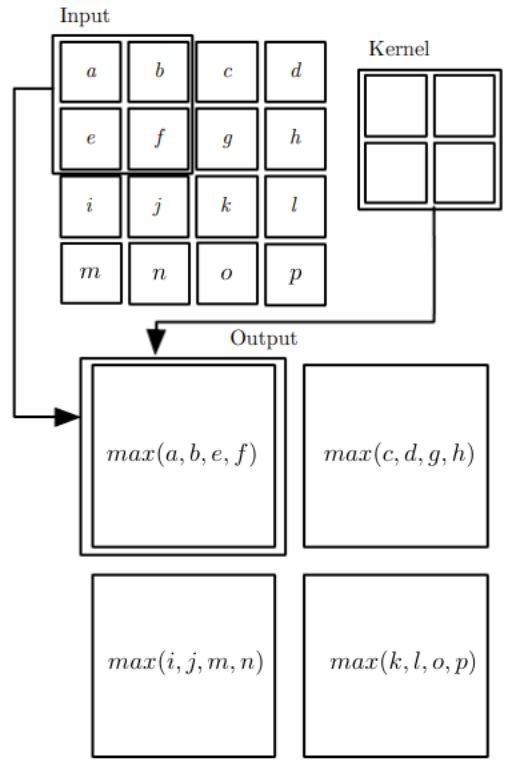
\includegraphics[scale=0.6]{Images/CNNArchitectures/maxpooling-operation.png}
	% 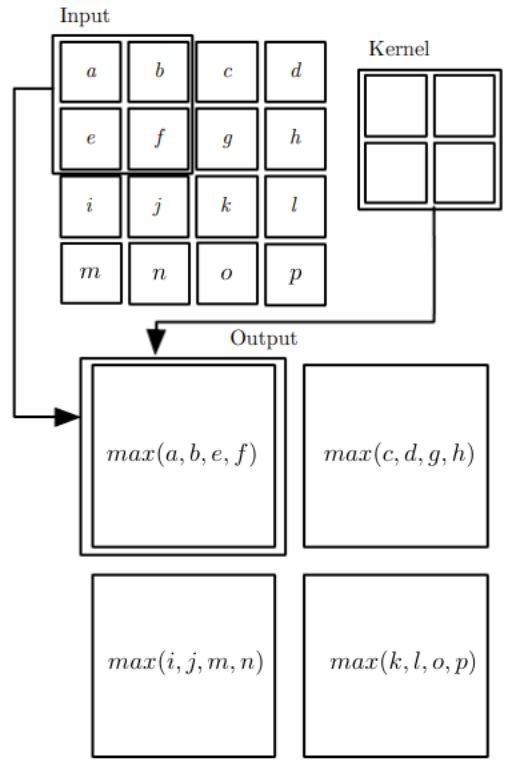
\includegraphics[width=\textwidth]{Images/CNNArchitectures/maxpooling-operation.png}
	\decoRule
	\caption[Max-Pooling Operation]{Max-Pooling Operation - A max operation is applied with a 2x2 Kernel on the 4x4 example input matrix with stride 2. Figure from \cite{Goodfellow-et-al-2016}.}
	\label{fig:max-pooling-operation}
\end{figure}

\subsubsection{Fully-Connected Layer}
The CNNs classifier part is comprised of several Fully-Connected layers, which serve as the high-level reasoning. It is the part that finally classifies the given input.

A Fully-Connected layer is the simplest type of layer, as it is the one used in Multi-Layer Perceptron (MLP) neural networks. More specifically, it receives input, with which it computes a weighted sum for each of its output values. This input is derived from the flattened output of several convolutional and pooling layers.

Each Fully-Connected layer is defined by its hyperparameters. Those are:
\begin{itemize}
	\item \textbf{Output Features:} The number of features to output. Consequently, this also configures the number of weights needed for the computation, hence, its memory and computation footprint.
\end{itemize}

The mathematical expression of the Fully-Connected layer's operation (Equation \ref{eqn:fully-connected}) is defined bellow.

Let \emph{I} be the input with \emph{N} input features, let \emph{W} be the layers weights, let \emph{B} be the layer's bias, and let \emph{M} be the layer's output features. So the Fully-Connected layer's output, \emph{Out}, is defined as:
\begin{equation}
	\label{eqn:fully-connected}
	Out(i) = B(i) + \sum_{j = 1}^{N} I(j)W(i, j), \mbox{for i = 1, 2, ..., M}
\end{equation}

The parameters' reuse of Fully-Connected layers from a specific application to another cannot be done since they are strictly bonded to the classes and high-level features of the particular Convolutional neural network.

The final Fully-Connected layers is typically followed by a Softmax activation layer, which, as stated on section \ref{subsection:ANNs-Basic-components}, it calculates the probability of the input being a certain class. The use of Softmax enables the confidence quantification for every estimation, and easy troubleshooting when the input it misclassified.

\subsubsection{Activation Layer}
There can be an activation layer after each Convolutional and Fully-Connected layer, which applies an activation function on the output of its previous layer. An activation layer increases the network's nonlinearity without affecting the convolutional layers' receptive fields. The activation function can be one of those presented in section \ref{subsection:ANNs-Basic-components}, but ReLU is generally preferred, due to its fast training characteristics and its low penalty on generalization accuracy.

\section{Theoretical knowledge sources}
The aforementioned theoretical background was mostly obtained from the Statistical Modeling and Pattern Recognition course of Electrical and Computer Engineering school at the Technical University of Crete. In addition, the book Deep Learning \cite{Goodfellow-et-al-2016} was used when finer details were needed. Moreover, the Udacity course Intro to Deep Learning with PyTorch by Facebook AI \cite{Udacity-Intro-to-Deep-Learning-with-PyTorch-by-Facebook-AI} was used for a more hands-on approach, focusing on PyTorch and Python in general. Last but not least, a great resource has been all the papers mentioned above.
